\documentclass[border=4pt]{standalone}
\usepackage{amsmath,amssymb}
\usepackage{tikz}
\begin{document}
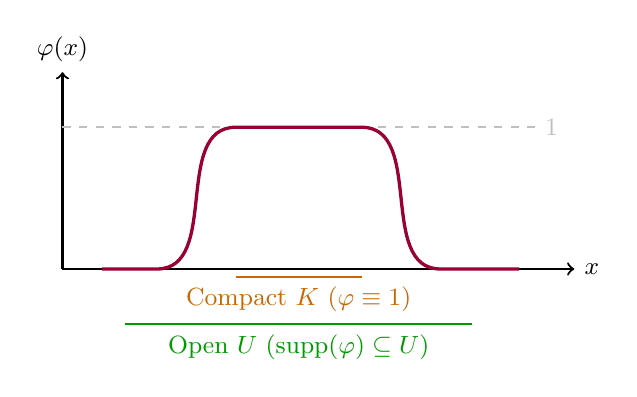
\begin{tikzpicture}[font=\small]
  \draw[->, thick] (0,0) -- (6.5,0) node[right] {$x$};
  \draw[->, thick] (0,0) -- (0,2.5) node[above] {$\varphi(x)$};

  \draw[thick, dashed, gray!50] (0, 1.8) -- (6.0, 1.8) node[right] {$1$};

  % Smooth bump curve
  \draw[very thick, purple!80!black] 
    (0.5, 0) -- (1.2, 0) 
    to[out=0, in=180] (2.2, 1.8) 
    -- (3.8, 1.8) 
    to[out=0, in=180] (4.8, 0) 
    -- (5.8, 0);

  % Brackets for K and U
  \draw[thick, orange!80!black] (2.2, -0.1) -- (3.8, -0.1) node[midway, below] {Compact $K$ ($\varphi \equiv 1$)};
  \draw[thick, green!60!black] (0.8, -0.7) -- (5.2, -0.7) node[midway, below] {Open $U$ ($\mathrm{supp}(\varphi) \subseteq U$)};
\end{tikzpicture}
\end{document}